\newpage

\section{Opracowanie wyników}

Strukturę $\mathbf{Ga_{2}S_{3}}$ można przedstawić w postaci grup $\mathbf{GaS_{4}}$. Siarka jest zlokalizowana na wierzchołkach tetraedru, a gal jest zlokalizowany w środku.

\begin{figure}[H]
	\begin{center}
		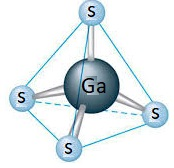
\includegraphics[width=0.3\linewidth]{Opracowanie/tetraedr.jpg}
		\caption{Grupa $\mathbf{Ga_{2}S_{3}}$.}
	\end{center}
\end{figure}

Przy takiej budowie krystalicznej fonony można podzielić na dwie grupy:
\begin{itemize}
	\item Fonony o niskiej energii. Niskoenergetycznych fonony położone są w widmie ramanowskim poniżej 200 $cm^{-1}$. Do tej grupy należą piki o numerach: 1, 2, 3;
	\item Fonony o wysokiej energii. Wysokoenergetyczne fononypołożone są w widmie ramanowskim powyżej 200 $cm^{-1}$. Do tej grupy należą piki o numerach 4, 5, 6, 7;
\end{itemize}

Przez analogię do oscylatora harmonicznego, częstotliwość drgań $\omega$ można przedstawić za pomocą wzoru:
\begin{equation}
	\omega = \sqrt{\frac{k}{m}}
\end{equation} 

\begin{itemize}
	\item $k$ -- stałą sprężystości, która zależy od siły oddziaływania między drgającym atomami;
	\item $m$ -- masa atomów.
\end{itemize}

Drgania atomów w obrębie jednego tetraedru odpowiada drganiom o wysokiej energii, dlatego że siły wiązania między cząsteczkami w tym samym tetraedrze są duże. Natomiast drgania w których uczestniczą całe tetraedry odpowiadają drganiom niskoenergetycznym ze względu na dużą masę drgających cząsteczek.

Przed rozpoczęciem pomiaru szukaliśmy pod mikroskopem pojedynczego kryształka który przypomina sześciokąt, ponieważ przy pomiarach kryształka w postaci sześciokąta można określić jego osie krystalograficzne i ich orientację w przestrzeni.

Chociaż mamy strukturę jednoskośną, przy określonym kierunku kryształ rośnie w postaci sześciokątów. Niżej zostały przedstawione struktury wygenerowane programem VESTA dla struktur $\alpha'$-$\mathbf{Ga_{2}S_{3}}$, $\alpha$-$\mathbf{Ga_{2}S_{3}}$ i  $\beta$-$\mathbf{Ga_{2}S_{3}}$:

\begin{center}
	\begin{figure}[H]
		\begin{minipage}[h]{0.47\linewidth}
			\center{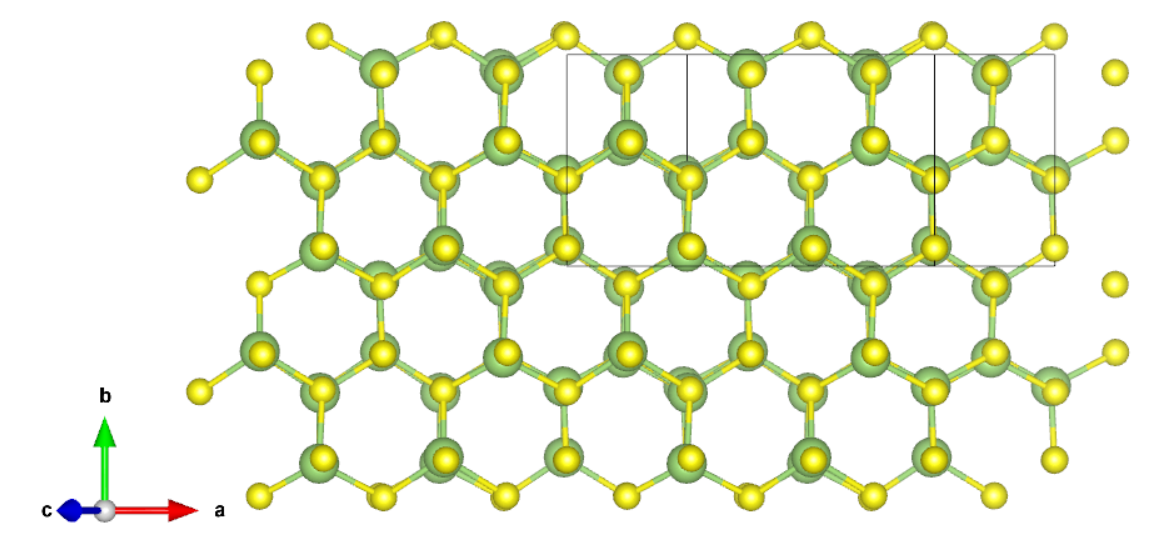
\includegraphics[width=0.8\linewidth]{Opracowanie/alfa_prim_Cc.png}} \\a)
		\end{minipage}
		\hfill
		\begin{minipage}[h]{0.47\linewidth}
			\center{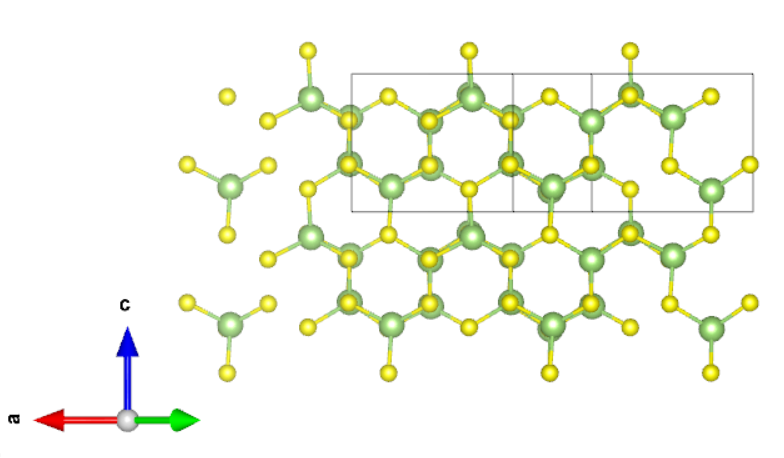
\includegraphics[width=0.8\linewidth]{Opracowanie/alfa_prim_Bb.png}} \\b)
		\end{minipage}
		\caption{a) Struktura krystaliczna $\alpha'$-$\mathbf{Ga_{2}S_{3}}$, grupa przestrzenna Cc. Osie krystalograficzne \textbf{a} i \textbf{b} są prostopadłe i leżą w jednej płaszczyźnie i odpowiadają osiom kartezjańskim x i y. Oś krystalograficzna \textbf{c} jest prostopadła do \textbf{b} i skierowana pod kątem 121$^{\circ}$ oraz pod kątem 31$^{\circ}$ do osi kartezjańskiej z. b) Struktura krystaliczna $\alpha'$-$\mathbf{Ga_{2}S_{3}}$, grupa przestrzenna Bb. Osie krystalograficzne \textbf{a} i \textbf{c} są prostopadłe i leżą w jednej płaszczyźnie i odpowiadają osiom kartezjańskim x i z. Oś krystalograficzna \textbf{b} jest prostopadła do \textbf{c} i skierowana pod kątem 141$^{\circ}$ do \textbf{a}, i skierowana pod kątem 51$^{\circ}$ do osi kartezjańskiej y. Przygotowano używając oprogramowanie VESTA [5].}
	\end{figure}
\end{center}

\begin{center}
	\begin{figure}[H]
		\begin{minipage}[h]{0.47\linewidth}
			\center{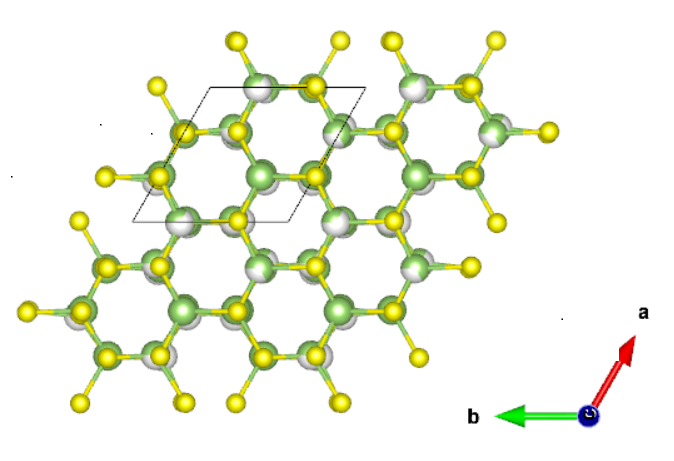
\includegraphics[width=0.8\linewidth]{Opracowanie/alfa.png}} \\a)
		\end{minipage}
		\hfill
		\begin{minipage}[h]{0.47\linewidth}
			\center{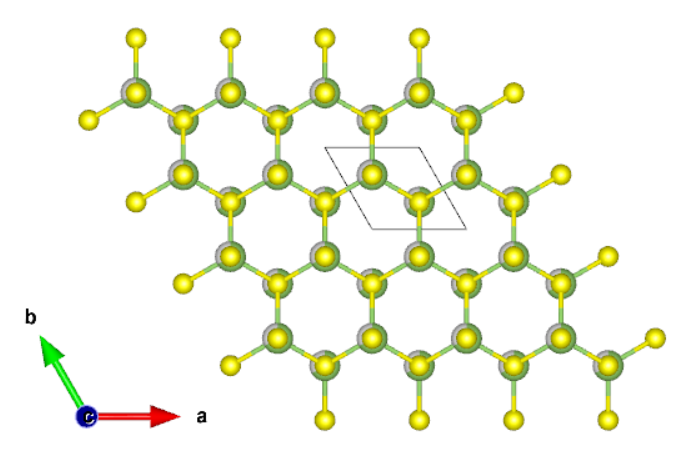
\includegraphics[width=0.8\linewidth]{Opracowanie/beta.png}} \\b)
		\end{minipage}
		\caption{a) Struktura krystaliczna $\alpha$-$\mathbf{Ga_{2}S_{3}}$. Osie krystalograficzne \textbf{a} i \textbf{b} są skierowane pod kątem 120$^{\circ}$ i leżą w jednej płaszczyźnie. Oś krystalograficzna a odpowiada osi kartezjańskiej x, a oś krystalograficzna \textbf{b} jest skierowana pod kątem 30$^{\circ}$ do osi kartezjańskiej y. Oś krystalograficzna c odpowiada osi kartezjańskiej z i jest prostopadła do płaszczyzny w której leżą \textbf{a} i \textbf{b}. b) Struktura krystaliczna $\beta$-$\mathbf{Ga_{2}S_{3}}$. Konfiguracja osi jest taka sama jak w a). Przygotowano używając oprogramowanie VESTA [5].}
	\end{figure}
\end{center}
	
Jak widać z rysunków praktyczna każda ze struktur krystalograficznych $\mathbf{Ga_{2}S_{3}}$ przy odpowiedniej orientacji osi krystalograficznych może prowadzić do kryształków, wyglądających jak sześciokąty. Z tego względu analiza modów fononowych dla różnych struktur pozwoliła wskazać fazę monoclinic (jednoskośną) jako najbardziej prawdopodobną w naszym przypadku. Istotne w tym przypadku były zależności polaryzacyjne pików ramanowskich.

Natężenie modu drgającego przy pobudzeniu wiązką laserową zmienia się według wzoru (1). Wektory polaryzacji $e_{i}$ i $e_{s}$ dla naszego układu pomiarowego (konfiguracja backscattering) można przedstawić dla konfiguracji VV i VH w postaci poniższych wzorów:
\begin{itemize}
	\item Dla konfiguracji VV wektory mają następującą postać:
	\begin{itemize}
		\item $e_{i} = [\cos \alpha, \sin \alpha, 0]$;
		\item $e_{s} = [\cos \alpha, \sin \alpha, 0]$.
	\end{itemize}
	\item Dla konfiguracji VH wektory mają następującą postać:
	\begin{itemize}
		\item $e_{i} = [\cos \alpha, \sin \alpha, 0]$;
		\item $e_{s} = [-\sin \alpha, \cos \alpha, 0]$.
	\end{itemize}
\end{itemize}

W naszym układzie pomiarowym wiązka padająca i rozproszona miała kierunek osi z, natomiast obrót polaryzacji wiązki padającej zachodził w płaszczyźnie x-y.

Tensory ramanowskie dla struktury jednoskośnej w takim układzie osi (x y z) są następujące:

\begin{figure}[H]
	\begin{center}
		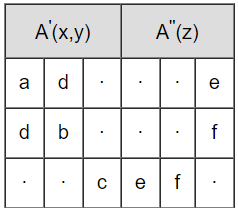
\includegraphics[width=0.3\linewidth]{Opracowanie/Tensor-Cc.png}
		\caption{Tensory ramanowskie dla struktury jednoskośnej.}
	\end{center}
\end{figure}

Z tego wynika, że w przypadku dla struktury jednoskośnej powinniśmy mieć do czynienia z modami o symetrii $A^{'}$ i $A^{''}$. Przy czym mody o symetrii $A^{''}$ nie powinny być widoczne w naszej konfiguracji pomiarowej.

Piki oznaczone numerami 1, 4, 7 zostały wybrane dla dopasowań, ponieważ natężenie tych pików w widmie ramanowskim jest stosunkowo duże, ponad to w otoczeniu tych pików nie występował żaden inny pik ramanowski, stąd one mogły być dopasowywane w postaci pojedynczej funkcji Voita. Taka sytuacja prowadzi do stosunkowo małych błędów dopasowania. 

Na kolejnych rysunkach przedstawiano zależności polaryzacyjne dla tych pików w konfiguracji VV oraz krzywe dopasowania, wykorzystując tensor ramanowski dla modu $A^{'}$. Przy każdym z rysunków podane zostały również uzyskane współczynniki tensora ramanowkiego.


\begin{figure}[H]
	\begin{center}
		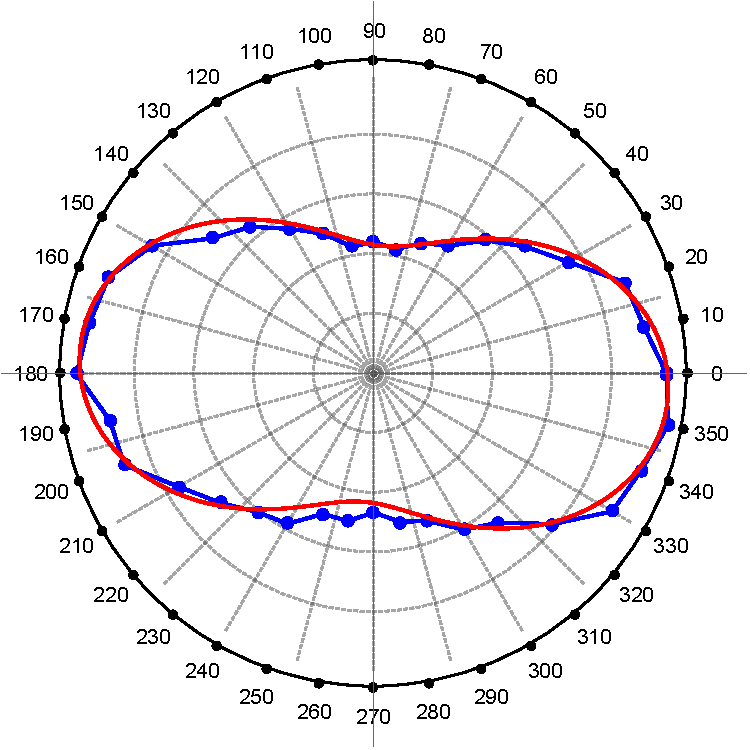
\includegraphics[width=0.5\linewidth]{Wyniki/WidmoPolaryzacyjne/Dopasowania/dopasowanieVV1.pdf}
		\caption{Zależność polaryzacyjna w konfiguracja VV dla modu oznaczonego numerem 1) (krzywa niebieska) oraz dopasowanie według wzoru 1) przy założeniu symetrii modu A$^{'}$ (krzywa czerwona). Uzyskane w wyniku dopasowania parametry tensora ramanowsiego: a = 1, b = 0.78, d = 0.12} 
	\end{center}
\end{figure}

\begin{figure}[H]
	\begin{center}
		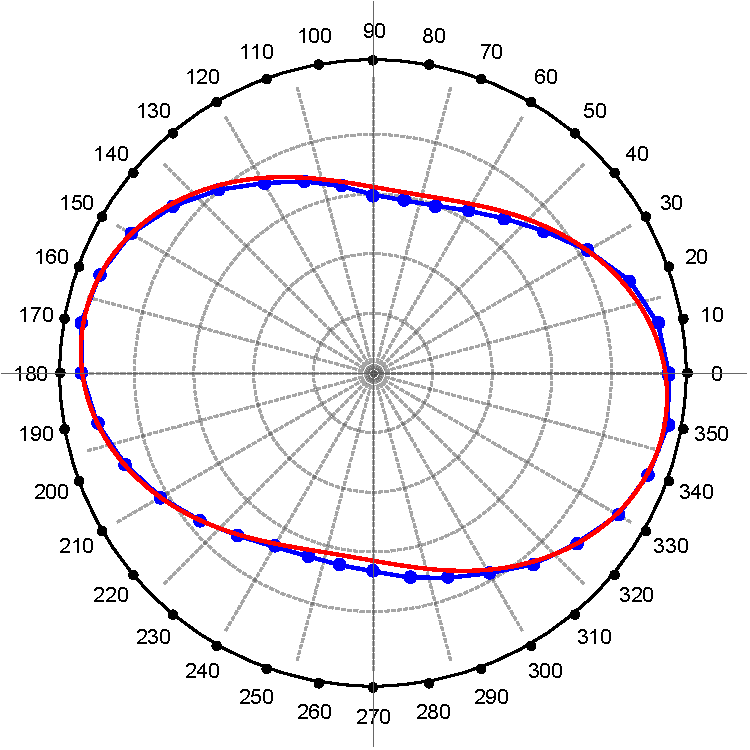
\includegraphics[width=0.5\linewidth]{Wyniki/WidmoPolaryzacyjne/Dopasowania/dopasowanieVV4.pdf}
		\caption{Zależność polaryzacyjna w konfiguracja VV dla modu oznaczonego numerem 4) (krzywa niebieska) oraz dopasowanie według wzoru 1) przy założeniu symetrii modu A$^{'}$ (krzywa czerwona). Uzyskane w wyniku dopasowania parametry tensora ramanowsiego: a = 1, b = 0.80, d = 0.10}
	\end{center}
\end{figure}

\begin{figure}[H]
	\begin{center}
		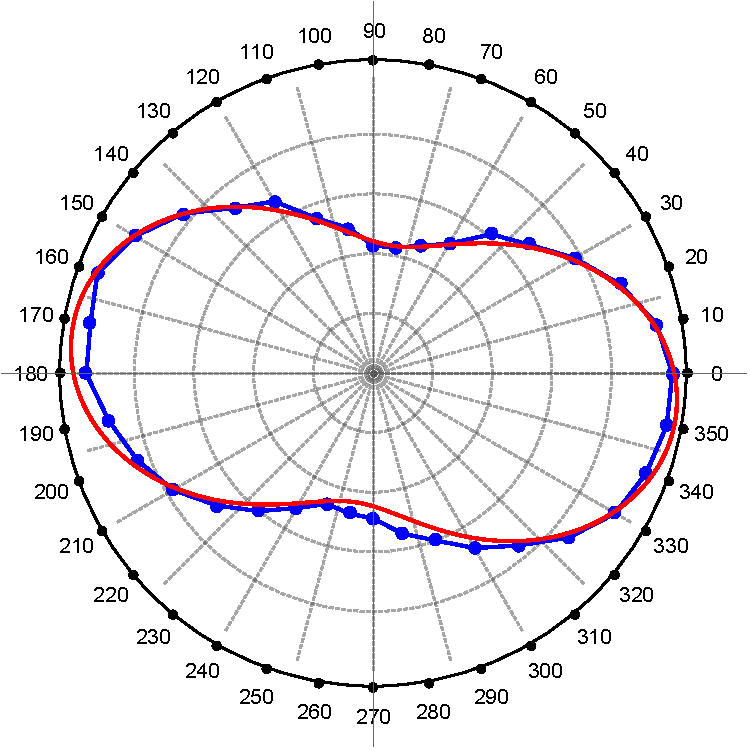
\includegraphics[width=0.5\linewidth]{Wyniki/WidmoPolaryzacyjne/Dopasowania/dopasowanieVV7.pdf}
		\caption{Zależność polaryzacyjna w konfiguracja VV dla modu oznaczonego numerem 7) (krzywa niebieska) oraz dopasowanie według wzoru 1) przy założeniu symetrii modu A$^{'}$ (krzywa czerwona). Uzyskane w wyniku dopasowania parametry tensora ramanowsiego: a = 1, b = 0.67, d = 0.12} 
	\end{center}
\end{figure}

Zależności polaryzacyjne i dopasowane krzywe zgadzają się z dużą dokładnością. Parametry tensora ramanowskiego, który odpowiada modu A$^{'}$ są następujące:
\begin{itemize}
	\item parametr $a$ przyjmuje wartość 1, parametr $b$ jest w granicach 0.67 - 0.80, 
	\item parametr $b$ przyjmuje wartości w granicach 0.67 - 0.80.
	\item parametr $d$ przyjmuje wartości w granicach 0.10 - 0.12.
\end{itemize}
Wyniki te były prezentowane na konferencji MRS.

Uzyskane dopasowania pozwalają z dużym prawdopodobieństwem określić, że mamy do czynienie z fazą jednoskośną. W przypadku innych struktur mamy do czynienia z modami o różnej symetrii.

Jeżeli chodzi o konfigurację VH na tym etapie pracy występowały pewne problemy z dopasowaniami. Wymaga to przeprowadzenia dodatkowych pomiarów sprawdzających. Badania związane z konfiguracją VH dla struktury $\alpha'$-$\mathbf{Ga_{2}S_{3}}$ będzie przedmiotem kolejnych prac.




